\section[粒子在库仑场中的运动(束缚态)]{粒子在库仑场中的运动(束缚态)} \label{sec:05.04} % 
% \makebox[5em][s]{} % 短题目拉间距

\blfootnote{* 涉及库仑力作用$e^{2}/4\pi\varepsilon_{0}$简记为$\e^{2}$}
电子在原子核的库仑场中形成的束缚态,是原子和分子结构的基础,以$Ze$表示原子核电荷,$-e$表示电子电荷,原子核对电子的库仑作用势$^{*}$为
\begin{empheq}{equation}\label{eq54.1}
	V(r)=-\frac{Z\e^{2}}{r}
\end{empheq}
如略去原子核的运动,则电子的哈密顿算符可以写成
\begin{empheq}{equation}\label{eq54.2}
	\hat{H}=\hat{T}+\hat{V}=-\frac{\hbar^{2}}{2\mu}\nabla^{2}-\frac{Z\e^{2}}{r}
\end{empheq}
$\mu$为电子质置\footnote{严格说,原子核-电子体系应该作为二体问题处理,\eqref{eq54.2}式是电子对于核的相对运动哈密顿算符,其中$\mu$为折合质量.详细讨论请看$\S$\ref{sec:10.01}}.根据$\S$\ref{sec:05.01}的讨论,$(\hat{H},\hat{\boldsymbol{L}}^{2},\hat{L}_{z})$的共同本征函数可以表示成
\begin{empheq}{equation}\label{eq54.3}
	\varPsi=R(r)Y_{lm}(\theta,\varphi)=\frac{u(r)}{r}Y_{lm}(\theta,\varphi)
\end{empheq}
代入能量本征方程
\begin{empheq}{equation*}
	\hat{H}\varPsi=E\varPsi
\end{empheq}
得到径向方程
\begin{empheq}{equation}\label{eq54.4}
	\frac{d^{2}u}{dr^{2}}+\bigg[\frac{2\mu E}{\hbar^{2}}+\frac{2\mu Z\e^{2}}{\hbar^{2}}\frac{1}{r}-\frac{l(l+1)}{r^{2}}\bigg]u=0
\end{empheq}
只讨论束缚态,$E<0$.$\S$\ref{sec:05.01}已经一般地证明$u(r)$具有近似性质
\begin{empheq}{align}\label{eq54.5}
	r&\rightarrow 0,u(r)\sim Cr^{l+1}	\nonumber\\
	r&\rightarrow\infty,u(r)\sim C_{3}e^{-\alpha r},\alpha=\frac{\sqrt{-2\mu E}}{\hbar}
\end{empheq}
因此,令
\begin{empheq}{equation}\label{eq54.6}
	u(r)=Cr^{l+1}F(r)e^{-\alpha r}
\end{empheq}
其中$C$为归一化常数,$F(r)$为待定函数,$r\rightarrow 0$处$F\rightarrow 1$,将变换\eqref{eq54.6}式代入\eqref{eq54.6}式,得到$F(r)$满足的方程为
\eqllong
\begin{empheq}{equation}\label{eq54.7}
	r\frac{d^{2}F}{dr^{2}}+(2l+2-2\alpha r)\frac{dF}{dr}+\bigg[\frac{2\mu Z\e^{2}}{\hbar^{2}}-(2l+2)\alpha\bigg]F=0
\end{empheq}\eqnormal
引入无量纲变量
\begin{empheq}{equation}\label{eq54.8}
	\xi=2\alpha r=\frac{2}{\hbar}\sqrt{-2\mu Er}
\end{empheq}
并用$2\alpha$除\eqref{eq54.7}式,可以简化成
\eqlong
\begin{empheq}{equation}\label{eq54.9}
	\xi\frac{d^{2}F}{d\xi^{2}}+(2l+2-\xi)\frac{dF}{d\xi}-\bigg(l+1-\frac{\mu Z\e^{2}}{\alpha\hbar^{2}}\bigg)F=0
\end{empheq}\eqnormal

{\heiti 合流超几何方程}

这种方程的一般形式是
\begin{empheq}{equation}\label{eq54.10}
	\xi F^{\prime\prime}+(b-\xi)F^{\prime}-aF=0
\end{empheq}
$a,b$为常数,$b$不等于负整数或零,满足边条件$F(0)=1$的解可以表示成
\begin{empheq}{equation}\label{eq54.11}
	F=\sum_{\nu=0}^{\infty}C_{\nu}\xi^{\nu}
\end{empheq}
代入\eqref{eq54.10}式,比较$\xi^{\nu}$项系数,可得递推关系
\begin{empheq}{equation}\label{eq54.12}
	C_{\nu+1}=\frac{a+\nu}{(b+\nu)(\nu+1)}C_{\nu}
\end{empheq}
从$\nu=0$开始,反复利用这关系,即得
\begin{empheq}{equation}\label{eq54.13}
	C_{\nu+1}=\frac{a(a+1)\cdots(a+\nu)}{b(b+1)\cdots(b+\nu)\cdot(\nu+1)!}
\end{empheq}
相应的$F(\xi)$记作
\eqindent{1}
\begin{empheq}{equation}\label{eq54.14}
	F(a,b,\xi)=1+\frac{a}{b}\xi+\frac{a(a+1)}{b(b+1)}\frac{\xi^{2}}{2!}+\frac{a(a+1)(a+2)}{b(b+1)(b+2)}\frac{\xi^{3}}{3!}+\cdots
\end{empheq}\eqnormal
称为合流超几何函数,$F(a,b,\xi)$是其专用符号.

\eqref{eq54.10}式的另一个独立解为$\xi^{1-b}F(a-b+1,2-b,\xi)$.

如果$a$不等于负整数或零,\eqref{eq54.14}式是一个无穷级数,其渐近行为和$e^{\xi}$相似.$e^{\xi}$的级数展开式是
\eqlong
\begin{empheq}{equation}\label{eq54.15}
	e^{\xi}=\sum_{\nu=0}\frac{\xi^{\nu}}{\nu!}=1+\xi+\frac{\xi^{2}}{2!}+\frac{\xi^{3}}{3!}+\cdots
\end{empheq}
\eqref{eq54.12}式中,当$\nu$很大时,$\frac{C_{\nu+1}}{C_{\nu}}\sim\frac{1}{\nu+1}$,刚好和\eqref{eq54.15}式中$\xi^{\nu+1}$项与$\xi^{\nu}$项系数之比相同,所以$F(a,b,\xi)$和$e^{\xi}$的渐近性质相似可以证明,当$\xi$为复变数时,$F(a,b,\xi)$的较精确的渐近表示式为\footnote{[苏]朗道.量子力学.上册.北京:高等教育出版社,1980.附录d}
\begin{empheq}{equation}\label{eq54.16}
	F(a,b,\xi)^{|\xi|\rightarrow\infty}\sim\frac{\Gamma(b)}{\Gamma(b-a)}(-\xi)^{-a}+\frac{\Gamma(b)}{\Gamma(a)}\xi^{a-b}e^{\xi}
\end{empheq}\eqnormal

回到径向方程\eqref{eq54.9},它相当于\eqref{eq54.10}式中
\begin{empheq}{equation}\label{eq54.17}
	a=l+1-\frac{\mu Z\e^{2}}{\alpha\hbar^{2}},\quad b=2l+2
\end{empheq}
\eqref{eq54.9}式符合条件$F(0)=1$的解为$F=F(a,b,\xi)$.因此
\begin{empheq}{equation}\label{eq54.18}
	u(r)=Cr^{l+1}F(a,b,\xi)e^{-\alpha r},\quad \xi=2\alpha r
\end{empheq}
当$r\rightarrow\infty$,$u(r)$的渐近表示为
\begin{empheq}{equation*}
	u(r)\sim C_{l}r^{l+1-a}e^{-\alpha r}+C_{2}r^{l+1+a-b}e^{\alpha r}\rightarrow\infty
\end{empheq}
不符合束缚态波函数的物理性质.为了保证$r\rightarrow\infty$处$u(r)\rightarrow 0$,合流超几何函数$F(a,b,\xi)$必须于某项处中断,退化成一个$n_{r}$次多项式.这时$r\rightarrow\infty$处\eqref{eq54.6}式中指数函数$e^{-\alpha r}$起决定性作用,保证$u(r)$指数式衰减,迅速趋于0.$F(a,b,\xi)$退化成$n_{r}$次多项式的条件显然是$a=-n$,即
\begin{empheq}{equation*}
	l+1-\frac{\mu Z\e^{2}}{\alpha\hbar^{2}}=-n_{r},\quad n_{r}=0,1,2,\cdots
\end{empheq}
亦即
\begin{empheq}{equation*}
	\frac{\mu Z\e^{2}}{\alpha\hbar^{2}}=n_{r}+l+1\equiv n
\end{empheq}
\begin{empheq}{equation}\label{eq54.19}
\alpha=\frac{\mu Z\e^{2}}{n\hbar^{2}}=\frac{Z}{na_{0}},\quad a_{0}=\frac{\hbar^{2}}{\mu \e^{2}}
\end{empheq}
$a_{0}$即著名的玻尔半径,利用$\alpha$和能量的关系$\alpha=\frac{\sqrt{-2\mu E}}{\hbar}$,即可得到能级公式
\begin{empheq}{equation*}
	E=-\frac{\hbar^{2}\alpha^{2}}{2\mu}=-\frac{1}{2\mu}\bigg(\frac{\hbar Z}{na_{0}}\bigg)^{2}
\end{empheq}
亦即
\begin{empheq}{equation}\label{eq54.20}
	\boxed{E_{n}=-\frac{1}{2n^{2}}\frac{\mu \e^{4}Z^{2}}{\hbar^{2}}=-\frac{Z^{2}\e^{2}}{2n^{2}a_{0}}}
\end{empheq}
其中
\begin{empheq}{equation}\label{eq54.21}
	n=n_{r}+l+1=1,2,3,\cdots
\end{empheq}
因为$n$决定能级,习惯上称为主量子数.但从上述推导可知,$n$并不是原始的量子数,它是由$l$和$n_{r}$构成的.$n_{r}$称为径向量子数,$l$称为角量子数,$m$称为磁量子数,它们都是原始的量子数,取值为
\eqllong
\begin{empheq}{equation}\label{eq54.22}
	n_{r}=0,1,2,\cdots;\quad l=0,1,2,\cdots;\quad m=0,\pm1,\pm2,\cdots,\pm l
\end{empheq}\eqnormal

径向波函数$R(r)$只和量子数$l,n_{r}$有关,通常记为$R_{nl}$
\eqlong
\begin{empheq}{equation}\label{eq54.23}
	R_{nl}(r)=\frac{u(r)}{r}=N_{nl}\xi^{l}F(-n,2l+2,\xi)e^{-\xi/2}
\end{empheq}\eqnormal
其中
\begin{empheq}{equation*}\label{eq54.8'}
	\xi=2\alpha r=\frac{2Z}{na_{0}}r	\tag{$5.4.8^{\prime}$}
\end{empheq}
$N_{nl}$为归一化常数.归一化条件为
\begin{empheq}{equation}\label{eq54.24}
	\int_{0}^{\infty}R^{2}r^{2}dr=\int_{0}^{\infty}u^{2}dr=1
\end{empheq}
可以求出
\eqlong
\begin{empheq}{equation}\label{eq54.25}
	N_{nl}=\bigg(\frac{Z}{a_{0}}\bigg)^{\frac{3}{2}}\frac{2}{n^{2}(2l+1)!}\bigg[\frac{(n+l)!}{(n-l-1)!}\bigg]^{\frac{1}{2}}
\end{empheq}
属于最低的两个能级的归一化径向波函数为

\begin{align}
	\shortintertext{$n=1,l=0,n_{r}=0$}
	&R_{10}=\bigg(\frac{Z}{a_{0}}\bigg)^{\frac{3}{2}}2e^{-Zr/a_{0}}	\label{eq54.26}\\
	\shortintertext{$n=2,l=0,n_{r}=1$}
	R_{20}=&\bigg(\frac{Z}{a_{0}}\bigg)^{\frac{3}{2}}\frac{\sqrt{2}}{4}\bigg(2-\frac{Zr}{a_{0}}\bigg)e^{-Zr/2a_{0}}	\label{eq54.27}\\
	\shortintertext{$n=2,l=1,n_{r}=0$}	&R_{21}=\bigg(\frac{Z}{a_{0}}\bigg)^{\frac{3}{2}}\frac{\sqrt{6}}{12}\frac{Zr}{a_{0}}e^{-Zr/2a_{0}}	\label{eq54.28}
\end{align}\eqnormal
总波函数用量子数$n,l,m$表记,
\begin{empheq}{equation}\label{eq54.29}
	\varPsi_{min}=R_{nl}(r)Y_{lm}(\theta,\varphi)
\end{empheq}
基态波函数$(nlm=100)$为
\begin{empheq}{equation}\label{eq54.30}
	\boxed{\varPsi_{100}=R_{10}Y_{00}=\bigg(\frac{Z^{3}}{\pi a_{0}^{3}}\bigg)^{1/2}e^{-Zr/a_{0}}}
\end{empheq}
这个波函数应用极广,读者应该牢记.

以下对波函数\eqref{eq54.29}式和能级公式\eqref{eq54.20}作一些物理讨论.

{\heiti 能级分布及简并度}

最低的能级是基态$(n=1)$能级
\begin{empheq}{equation}\label{eq54.31}
	E_{1}=-\frac{\mu e^{4}Z^{2}}{2\hbar^{2}}=-\frac{Z^{2}e^{2}}{2a_{0}}
\end{empheq}
$E_{\infty}-E_{1}=|E_{1}|$就是基态电离能,即将电子从基态激发到游离态所需最小能量.对于氢原子$(Z=1)$,$|E_{1}|=13.6\si{eV}$,对于重元素,由于$Z$很大,$|E_{1}|$可达$10^{4}\si{eV}$量级.用$|E_{1}|$作为标准,能级公式可以写成
\begin{empheq}{equation*}
	E_{n}=\frac{E_{1}}{n^{2}},\quad n=1,2,3,\cdots
\end{empheq}
当$n\rightarrow\infty$,$E_{n}\rightarrow 0^{-}$,大量能级密集在$E=0$附近.

对于一个给定的能级$E_{n}$,角量子数$l$可取
\begin{empheq}{equation*}
	l=0,1,2,\cdots,(n-1)
\end{empheq}
对于某一种$l$,磁量子数$m$又有$(2l+1)$种取值.所以,与能级互相应的独立状态数为
\begin{empheq}{equation}\label{eq54.32}
	f_{n}=\sum_{l=0}^{n-1}(2l+1)=n^{2}
\end{empheq}
这就是能级$E_{n}$的简并度,也是中心力问题中最大的能级简并度,相当于图\ref{fig.5-1}中各组能级均与$l=0$这一组能级重合.(各组能级的起点随$l$之增大而升高)注意基态能级是不简并的.

{\heiti 径向概率分布}

以正电荷$(r=0)$为中心,将空间划分成许多同心球壳层,电子在$r-r+dr$层中出现概率为
\begin{empheq}{equation}\label{eq54.33}
	r^{2}dr\int|\varPsi_{nlm}|^{2}d\Omega=R^{2}r^{2}dr=u^{2}dr
\end{empheq}
因此,$r^{2}R^{2}=u^{2}$称为径向概率密度.如果$\varPsi_{nlm}$是原子外层电子的波函数,$u^{2}$最大值所对应的$r$值称为原子的最概然半径,简称原子半径.例如,对于氢原子的基态$(Z=1,nlm=100)$
\begin{empheq}{equation*}
	u(r)=rR_{10}(r)=Are^{-r/a_{0}}
\end{empheq}
$u^{2}$的极大值满足条件
\begin{empheq}{equation*}
	\frac{d}{dr}u^{2}=2u\frac{du}{dr}=0
\end{empheq}
即
\eqshort
\begin{empheq}{equation}\label{eq54.34}
	\frac{du}{dr}=0
\end{empheq}\eqnormal
由此求得$r=a_{0}$,这就是氢原子的基态半径(玻尔半径).玻尔量子论也给出同样的结果必须指出,量子力学关于原子形状的概念是和玻尔量子论不同的.按照玻尔量子论,氢原子中电子的基态轨道是一条圆形轨道,半径$a_{0}$,因此原子的形状像一个圆环.按照量子力学,氢原子的基态波函数$\varPsi_{100}(r)$是各向同性的,电子在各个方向出现概率相同,因此原子的形状像棉花球或球状的云,径向概率密度最大的球层半径就是原子半径.

在不同的场合,原子半径可以有不同的定义.例如电子与原子核间距离$r$的平均值
\begin{empheq}{equation}\label{eq54.35}
	\bar{r}=\int_{0}^{\infty}rR^{2}r^{2}dr=\int_{0}^{\infty}ru^{2}dr
\end{empheq}
经常被认为就是原子的有效半径.不同定义下的原子半径量级相同,数值稍有差异.例如对于氢原子的基态$\varPsi_{100}$,最概然半径为$a_{0}$,而$\bar{r}=\frac{3a_{0}}{2}$.

\begin{figure}[!h]
	\centering
	\small
	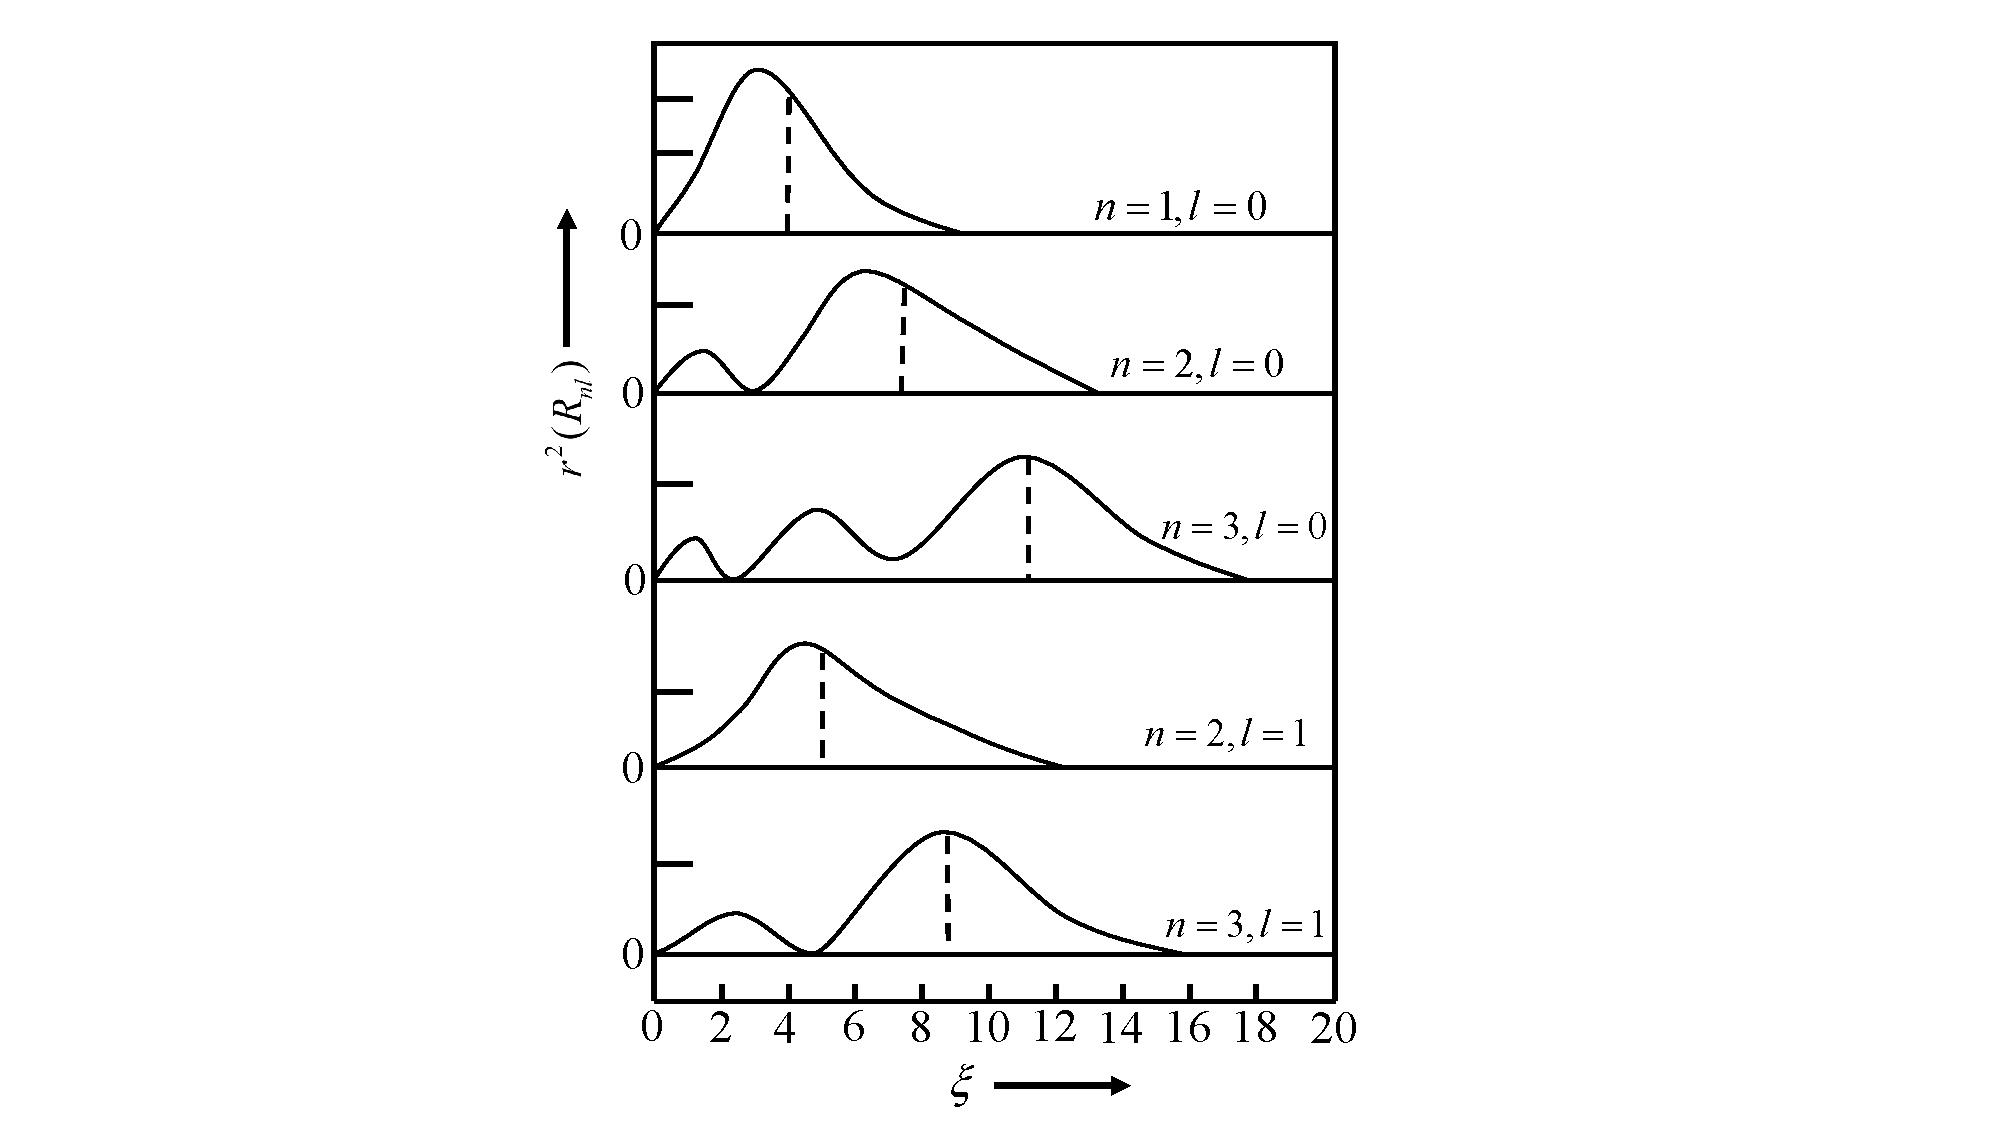
\includegraphics[width=5cm,clip]{QM file/figure/5-4}
	\caption{径向概率分布}\label{fig.5-4}
	\caption*{{\footnotesize 横坐标$\xi=\frac{2Zr}{na_{0}}$,虚线$\vdots$标出了$\bar{r}$的值.曲线的最高点所相应的$\xi$值即最概然半径}}
\end{figure}
在\eqref{eq54.3}式描述的状态下,任何$r$的函数(作为物理量)$G(r)$的平均值显然是
\begin{empheq}{equation}\label{eq54.36}
	\bar{G}=\int_{0}^{\infty}G(r)R^{2}r^{2}dr=\int_{0}^{\infty}G(r)u^{2}(r)dr
\end{empheq}
$\varPsi_{nlm}$态下电子的径向概率分布如图\ref{fig.5-4}所示.

{\heiti 角分布}

波函数$\varPsi_{nlm}$所反映的空间概率分布一般具有方向性.在任何一个球壳层内,电子在方向$(\theta,\varphi)$附近,立体角元$d\Omega=\sin\theta d\theta d\varphi$内出现概率比例于
\begin{empheq}{equation}\label{eq54.37}
	|Y_{lm}(\theta,\varphi)|^{2}d\Omega=A_{lm}^{2}|P_{l}^{m}(\cos\theta)|^{2}d\Omega
\end{empheq}
例如对于$l=1,m=1$的状态$\varPsi_{n11}$,由于$P_{1}^{1}=\sin\theta$,电子的角分布概率密度与$\sin^{2}\theta$成比例,电子出现概率最大的方向是$\theta
=\frac{\pi}{2}$,即$x-y$平面.s态$(l=0)$波函数$\varPsi_{n00}$与$\theta,\varphi$无关,电子的空间概率分布是各向同性的.

{\heiti 和玻尔量子论的比较}

以氢原子为例,将玻尔量子论的主要结果和量子力学结果作一比较.在玻尔量子论中,关于电子稳定轨道的计算同时应用了牛顿力学和量子化条件.根据牛顿力学,在库仑力作用下,电子的运动轨道是圆或椭圆,正电荷(原子核)位于圆心或椭圆的焦点.电子运动的能量$E$,轨道角动量$\boldsymbol{L}$,运行周期$\tau$和轨道的长半径$a$,短半径$b$(圆轨道$b=a$)之间有关系\footnote{钱伯初.行星轨道问题和玻尔量子论.大学物理.1985,6:7}
\begin{empheq}{align}	%38,39,40\label{eq54.3}
	E&=-\frac{e^{2}}{2a}		\label{eq54.38}\\
	\boldsymbol{L}^{2}=-2\mu& Eb^{2}=\frac{\mu e^{2}b^{2}}{a}		\label{eq54.39}\\
	\tau=\frac{2\pi\mu ab}{L},&\quad \tau^{2}=\frac{4\pi^{2}\mu a^{3}}{e^{2}}		\label{eq54.40}
\end{empheq}
量子化条件为
\begin{empheq}{equation}\label{eq54.41}
	L=n_{\varphi}\hbar,\quad n_{\varphi}=1,2,3,\cdots
\end{empheq}
由于能量$E$只和长半径$a$有关,当能量确定后,轨道的短半径仍有多种取值.角动量$\boldsymbol{L}$与短半径$b$成正比,而以圆轨道的角动量为最大.如以$n$表示圆轨道的角动量量子数$(\boldsymbol{L}=n\hbar)$,$a_{n}$表示其半径,$E_{n}$表示其能量,由\eqref{eq54.39}、\eqref{eq54.41}式易得
\begin{empheq}{equation}\label{eq54.42}
	a_{n}=\frac{n^{2}\hbar^{2}}{\mu e^{2}}=n^{2}a_{0},\quad n=1,2,\cdots
\end{empheq}
代入\eqref{eq54.38}式,得到能级
\begin{empheq}{equation}\label{eq54.43}
	E_{n}=-\frac{e^{2}}{2a_{n}}=-\frac{e^{2}}{2n^{2}a_{0}}
\end{empheq}
属于能级$E_{n}$的各种稳定轨道,长半径相同,均为$a_{n}$,角动量和短半径为
\begin{empheq}{align}	%44,45\label{eq54.4}
	L=n_{\varphi}\hbar,\quad n_{\varphi}&=n,n-1,\cdots,1		\label{eq54.44}\\
	b=\frac{n_{\varphi}}{n}a_{n}&=nn_{\varphi}a_{0}		\label{eq54.45}
\end{empheq}
总之,每一条稳定轨道的形状,由量子数$n,n_{\varphi}$标志,但能量仅与$n$有关.电子沿这样的稳定轨道运动时,等效的电流和磁矩为

\begin{empheq}{equation*}
	\text{电流}|I|=\frac{e}{\tau}=\frac{eL}{2\pi\mu ab}
\end{empheq}	\eqlong
\begin{empheq}{align}\label{eq54.46}
	\text{磁矩}|M|&=\frac{|I|}{c}\pi ab=\frac{eL}{2\mu c}	\nonumber\\
	&=n_{\varphi}\frac{e\hbar}{2\mu c}=n_{\varphi}\mu_{B}\quad\text{(高斯单位制)}
\end{empheq}\eqnormal
$\mu_{B}=\frac{e\hbar}{2\mu c}$为玻尔磁子.

如再考虑空间量子化(轨道法线的空间指向的量子化),还应该有
\begin{empheq}{align}	%47,48
	L_{z}=m\hbar,\quad m=0,&\pm1,\cdots,\pm n_{\varphi}		\label{eq54.47}\\
	M_{z}=-\frac{e}{2\mu c}L_{z}&=-m\mu_{B}		\label{eq54.48}
\end{empheq}

以上是玻尔量子论的主要结果,它和量子力学结果有相同之处,也有差异,列举如下:

(1) 能级公式,两种理论给出的结果相同.

(2) 就角量子数($l$或$n_{\varphi}$)与主量子数$n$的关系而言,$n_{\varphi}$相当于$(l+1)$.量子力学中$l$的最大值$l=(n-1)$所对应的状态相当于玻尔圆轨道.

(3) 就$L_{z}$的本征值而言,两种理论均给出
\begin{empheq}{equation*}
	L_{z}=m\hbar,\quad m=0,\pm1,\pm2,\cdots
\end{empheq}
但两种理论关于$\boldsymbol{L}^{2}$的本征值给出不同的结果,
\begin{empheq}{equation*}
	{\boldsymbol{L}^{2}=}
	\begin{dcases}
		n_{\varphi}^{2}\hbar^{2}	\quad\qquad\text{(玻尔量子论)}	\\
		l(l+1)\hbar^{2}	\quad \text{(量子力学)}
	\end{dcases}
\end{empheq}
当量子数较小时,两种结果有本质的差异,可以认为是不确定度关系起了重要作用.当量子数很大时,大致可以认为$n_{\varphi}$,相当于$\bigg(l+\frac{1}{2}\bigg)$.但就$L_{z}$的最大值而言,则$n_{\varphi}$相当于$l$.总之,$n_{\varphi}$和$l$的对应关系视着眼点之不同而稍有差异.

(4) 磁矩与角动量的关系,两种理论结果相同(量子力学理论见$\S$\ref{sec:05.01})但两种理论关于原子中由于电子运动而形成的电流分布,给出不同的结论.按照玻尔量子论,每一条稳定轨道相当于一个电流环(圆形或椭圆形).而量子力学结果($\S$\ref{sec:05.01})则是,当电子处于$\varPsi_{nlm}$态时,在空间任何地点,沿纬线方向均有电流存在.按照\eqref{eq51.28}式(取$q=-e$),
\begin{empheq}{equation*}
	j_{\varphi}=-m\frac{e\hbar}{\mu}\frac{\varPsi^{*}\varPsi}{r\sin\theta}
\end{empheq}
电流呈环状分布,以$z$轴为对称轴.

(5) 关于电子的空间位置,两种理论有着根本概念上的差异,在玻尔量子论中,电子的轨道是一条平面闭合曲线.如果是圆轨道,电子至原子核的相对距离是固定不变的.按照量子力学,在$\varPsi_{nlm}$态下,电子在全空间有一种概率分布.即使是$l$取最大值$(l=n-1)$的状态,电子仍可以在各种径向距离$(r)$上出现.但是,可以证明(习题5-11)对于$l=n-1$的状态,最概然半径等于$n^{2}a_{0}$,刚好等于玻尔圆轨道半径.

(6) 玻尔量子论中,不存在角动量$L=0$的稳定轨道.而在量子力学中,$l=0$的状态($s$态)常常是最重要的状态.能量最低的基态就是s态,由于$l=m=0$,波函数是实函数,电流和磁矩均等于0,而按照玻尔量子论,电子的基态轨道为圆形$(n=n_{\varphi}=1)$,等效磁矩等于$\mu_{B}$(玻尔磁子).实验已经判明,量子力学关于基态的结论$(l=m=0)$,磁矩为0,概率分布各向同性,等等)是正确的.

微妙的是,氢原子的基态$(nlm=100)$既是$l=0$的状态,又是$l$取最大值$(l=n-1=0)$的状态,在后一种意义上, 基态具有某些玻尔圆轨道的性质(如最概然半径刚好等于玻尔半径$a_{0}$),也就可以理解了.

{\heiti 物理模型}

由电荷异号的两个粒子(质量$m_{1},m_{2}$,电荷$q_{1},q_{2}$)构成的体系,如粒子间的作用主要是库仑作用,其他作用力可以忽略,则描述这两个粒子相对运动的哈密顿算符可以表示成
\begin{empheq}{equation}\label{eq54.49}
	\hat{H}=-\frac{\hbar^{2}}{2\mu}\nabla^{2}+\frac{q_{1}q_{2}}{r}\quad(q_{1}q_{2}<0)
\end{empheq}
其中$r$为相对坐标,$\mu=\frac{m_{1}m_{2}}{m_{1}+m_{2}}$是折合质量.与\eqref{eq54.2}式相比,相当于$Z\e^{2}$换成$|q_{1}q_{2}|$,$\mu$换成折合质量.所以,只要在波函数中也作相应的代换,本节的结果就可应用于这个二粒子体系。这样的体系有

氢原子-原子核为质子,电荷$q_{1}=+e$.电子电荷$q_{2}=-e$.

类氢离子-由原子核(电荷$q_{1}=Ze$)和一个电子构成,如$\ce{He}^{+},\ce{Li}^{++}$.

$\mu$原子-由原子核(电荷$q_{1}=Ze$)和一个$\mu$子(电荷$q_{2}=-e$)构成.$\mu$子质量为电子的207倍,其他性质与电子基本相同.

电子偶素-正、负电子$(e^{+},e^{-})$形成的束缚态.正电子$(e^{+})$是电子$(e^{-}$的反粒子,电荷$q_{1}=+e$,质量与电子相同.

还有一些问题,可以用本节的结果作为良好近似.例如,多电子原子(原子核电荷$Ze$)中的最内层($k$层)电子,所受作用力主要来自原子核,其状态很接近于由\eqref{eq54.30}式表示的基态$\varPsi_{100}$.又如,单价原子中最外层的价电子,所受作用势(原子核和内层电子库仑作用的总和)接近于$-\frac{\e^{2}}{r}$,价电子的波函数接近于氢原子的基态波函数$\varPsi_{100}$,但近似程度稍差.

\example 对于类氢离子的$\varPsi_{nlm}$态,计算离心势能的平均值.

\solution 径向方程\eqref{eq54.4}可以等效地看作一维定念薛定谔方程,能量算符相当于
\eqlong
\begin{empheq}{equation}\label{eq54.50}
	\hat{H}\Rightarrow-\frac{\hbar^{2}}{2\mu}\frac{d^{2}}{dr^{2}}+l(l+1)\frac{\hbar^{2}}{2\mu r^{2}}-\frac{Z\e^{2}}{r}=\hat{H}(l,r)
\end{empheq}\eqnormal
$u(r)$相当于波函数.视$l$为参数,则
\begin{empheq}{equation*}
	\frac{\partial\hat{H}}{\partial l}=(2l+1)\frac{\hbar^{2}}{2\mu r^{2}}
\end{empheq}
按照海尔曼定理($\S$\ref{sec:03.11}),应有
\begin{empheq}{equation}\label{eq54.51}
	\bigg\langle\frac{\partial\hat{H}}{\partial l}\bigg\rangle_{min}=\frac{\partial}{\partial l}E_{nlm}
\end{empheq}
今已知
\eqlong
\begin{empheq}{equation*}
	E_{nlm}=E_{n}=-\frac{1}{2n^{2}}\frac{\mu \e^{4}Z^{2}}{\hbar^{2}},\quad n=l+n_{r}+1
\end{empheq}
代入\eqref{eq54.51}式, 即得
\begin{empheq}{equation*}
	\frac{(2l+1)\hbar^{2}}{2\mu}\bigg\langle\frac{1}{r^{2}}\bigg\rangle_{min}=\frac{\partial E_{n}}{\partial l}=\frac{\partial E_{n}}{\partial n}=\frac{\mu \e^{4}Z^{2}}{n^{3}\hbar^{2}}
\end{empheq}\eqnormal
亦即
\begin{empheq}{equation}\label{eq54.52}
	\bigg\langle\frac{1}{r^{2}}\bigg\rangle_{min}=\frac{Z^{2}}{n^{3}\bigg(1+\frac{1}{2}\bigg)a_{0}^{2}}
\end{empheq}
离心势能平均值为
\eqlong
\begin{empheq}{equation}\label{eq54.53}
	\bigg\langle\frac{l(l+1)\hbar^{2}}{2\mu r^{2}}\bigg\rangle_{min}=\frac{l(l+1)Z^{2}\e^{2}}{(2l+1)n^{3}a_{0}}=-\frac{l(l+1)}{\bigg(l+\frac{1}{2}\bigg)n}
\end{empheq}\eqnormal
由于$(-E_{n})$等于动能平均值,所以在动能中离心势能所占比例为$\frac{l(l+1)}{\bigg(l+\frac{1}{2}\bigg)n}$.当$n$给定后,$l$越大,这个比例越大,当$l$取最大值$(n-1)$,这个比例为$\frac{n-1}{n-\frac{1}{2}}$,这时径向动能仅占动能的$\frac{1}{2n-1}$.所以,如$n\geqslant 1$,在$(n,n-1,m)$态中径向动能所占比例很小,这种状态相当于玻尔圆轨道.(牛顿力学中圆轨道$r$不变,径向动能为0.)